\chapter{Literature Review}
\label{ch:literaturereview}

\section{Methodic Product Development}
\label{sec:methodicproductdevelopment}

Methodic product development by Pahl and Beitz underscores the necessity of a structured design procedure that not only fosters creativity and inventiveness but also ensures objective evaluation of outcomes. By amalgamating insights from design science, cognitive psychology, and practical experience, Pahl and Beitz's approach to systematic design methodology guides designers in navigating the complexities of technical systems, facilitating the transition from intuitive to purposeful paths and leading to more successful and comprehensible design outcomes. \cite{Pahl07j}

At the core of the Pahl and Beitz methodology is the understanding that effective product development involves a series of well-defined and interconnected stages \cite{Pahl07k}. They describe the product development process as a series of stages, each with its own defined objectives and activities. The four main stages are:

\textbf{Planning and Task Clarification:} The process begins with precise planning and task definition, involving collaboration with the marketing or dedicated planning unit. Regardless of origin, whether a product proposal or customer request, a deep understanding of the task is crucial. Detailed insights into prerequisites, constraints, and their significance lead to a comprehensive requirements list—a foundation for subsequent stages.

\textbf{Conceptual Design:} Building on this clarity, the conceptual design phase is pivotal. It seeks a fundamental solution by abstracting functions, identifying working principles, and integrating them into a cohesive structure. This culminates in defining a principle solution, encapsulating the design vision's essence.

\textbf{Embodiment Design:} Transitioning to concrete realization, embodiment design takes the forefront. Guided by technical and economic considerations, designers shape the construction structure. Multiple preliminary layouts assess design strengths and weaknesses, leading to the selection of the most promising variant.

\textbf{Detail Design:} The methodology's apex is the detail design phase, focusing on individual components. Precise arrangements, dimensions, materials, and other aspects are defined. Careful estimation of production possibilities and costs results in comprehensive production documentation, underlining the phase's importance in shaping the overall outcome.

Figure \ref{fig:pahlprocess} illustrates the Pahl and Beitz design process, highlighting the iterative nature of the methodology.


\begin{figure}[ht!]
    \centering
    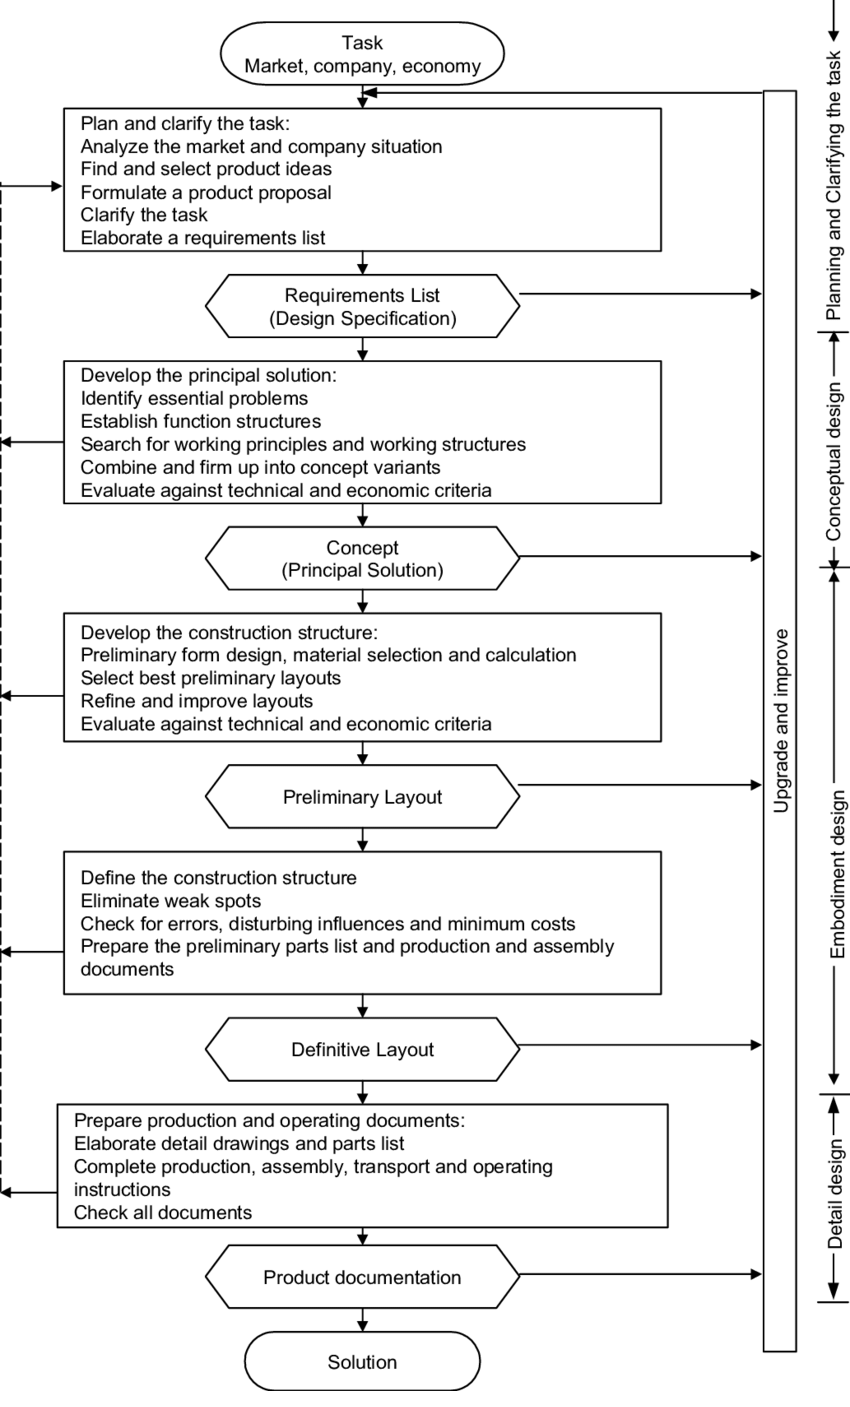
\includegraphics[width=0.8\textwidth]{texs/Part1/chapter1/image/pahlprocess.png}
    \caption{Pahl and Beitz's Design Process \cite{Pahl07l}}
    \label{fig:pahlprocess}
\end{figure}

\section{Fused Deposition Modeling}
\label{sec:fused_deposition_modeling}

Fused deposition modeling (FDM) is a widely used technique in additive manufacturing, particularly in 3D printing. It offers several advantages that contribute to its popularity in various industries. One of the main advantages of FDM is its ability to reproduce complex geometries with high precision and accuracy \cite{Gordeev18}.

This makes it suitable for creating intricate and customized designs that may not be achievable with traditional manufacturing methods. Additionally, FDM is a cost-effective process as it reduces material waste by only depositing the necessary amount of material layer by layer \cite{Gordeev18}. This not only saves costs but also promotes sustainability in manufacturing.

Common plastics used in FDM include acrylonitrile butadiene styrene (ABS), polylactic acid (PLA), and polyethylene terephthalate (PET) \cite{Teamm17}. Each of these materials has its own set of advantages and disadvantages that make them suitable for different applications.

To achieve a high quality printing result, there are several parameters that need to be considered. Takahashi et al. \cite{Takahashi17} classified these parameters into four categories: (1) operation parameters, (2) machine parameters, (3) machine parameters, and (4) geometry-specified parameters.

\subsection{Prusa Slicer i3 MK3S+}
\label{subsec:prusa_slicer}

The Prusa Slicer i3 MK3S+ is an FDM 3D printer designed for desktop use, ideal for tasks like rapid prototyping and small-scale production. With a build volume of 250 x 210 x 200 mm, it can achieve layer heights ranging from 0.05 mm to 0.35 mm \cite{Prusa}. Utilizing Cartesian printing and a single extruder, this printer comes equipped with a heated bed and is compatible with a diverse range of materials such as PLA, ABS, PETG, and nylon \cite{Prusa}. The default nozzle size is 0.4 mm, although alternate sizes can be utilized based on specific printing needs.

This 3D printer is accessible for use by both students and faculty members at the University of Applied Sciences Brandenburg and will play a pivotal role in the prototype development process. Figure \ref{fig:prusa_slicer_mk3} provides a visual representation of the Prusa Slicer i3 MK3S+, located within the Workshop of the University of Applied Sciences Brandenburg.

\begin{figure}
    \centering
    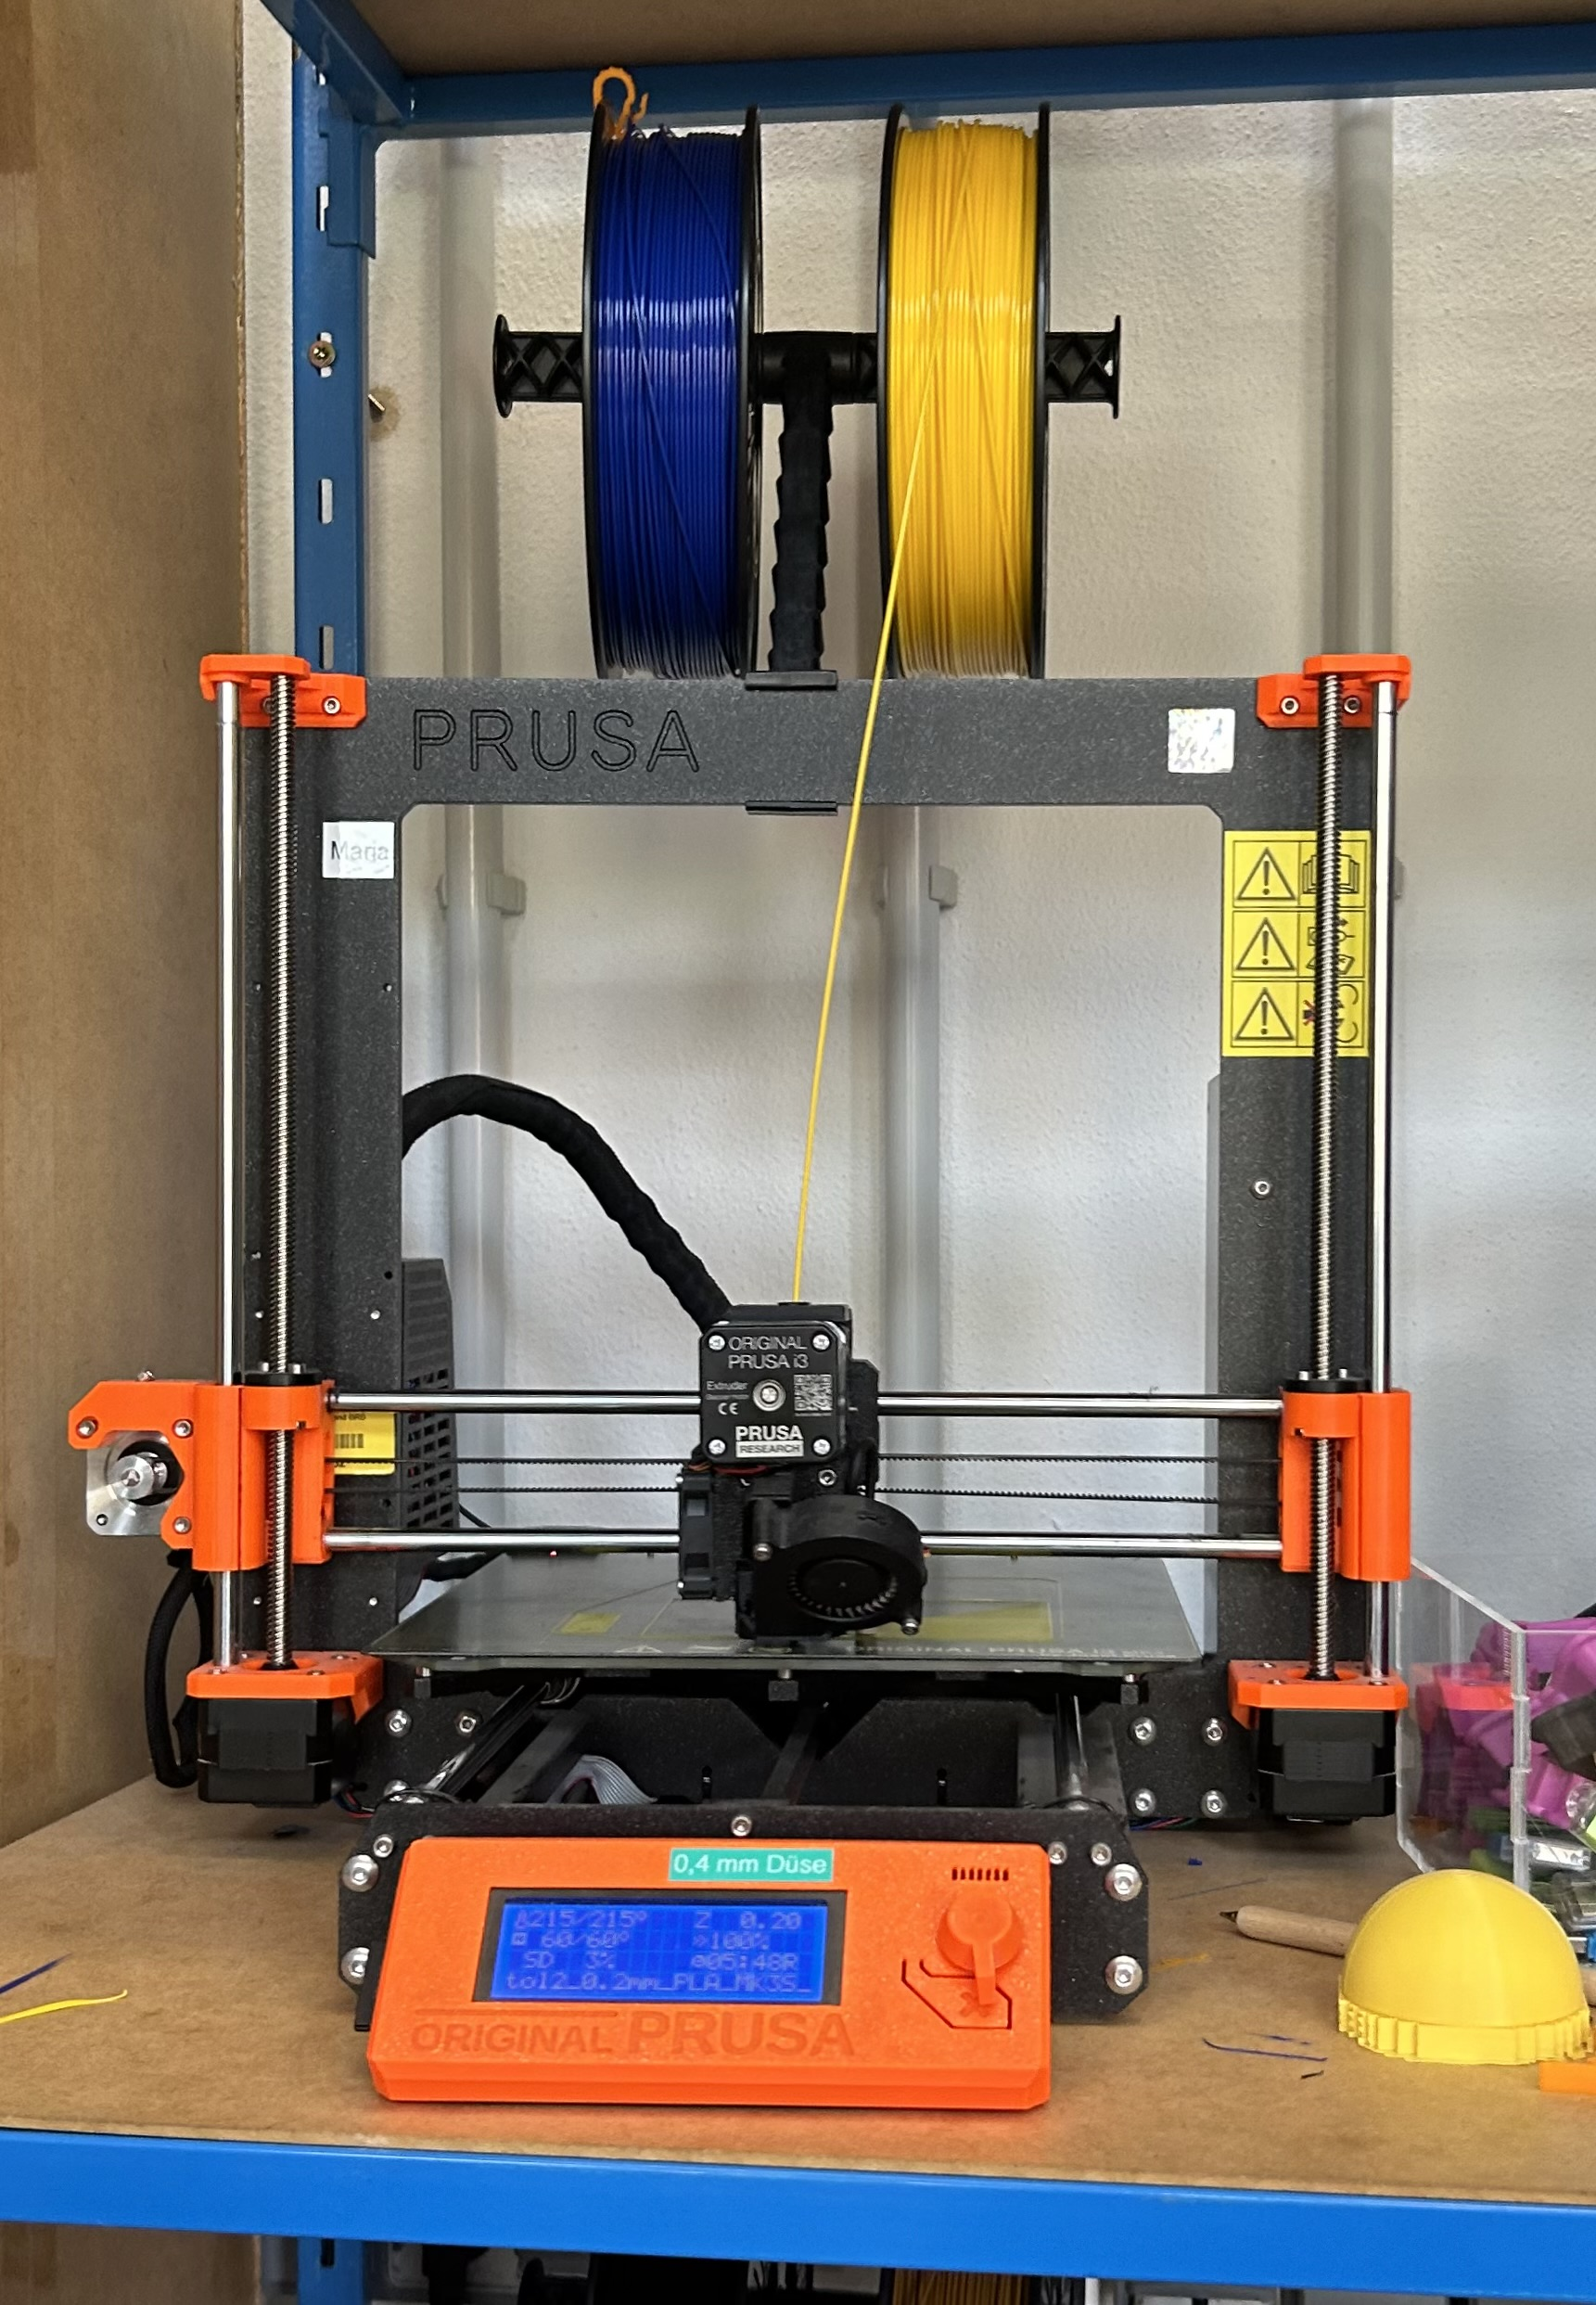
\includegraphics[height=8cm]{texs/Part1/chapter1/image/prusa.jpg}
    \caption{Prusa Slicer i3 MK3S+}
    \label{fig:prusa_slicer_mk3}
\end{figure}

\subsection{PrusaSlicer}
\label{subsec:prusa_slicer}

PrusaSlicer is a free and open-source slicing software that converts 3D models into G-code, a language that instructs the 3D printer on how to print the object. It is compatible with a wide range of 3D printers and supports a variety of filament materials. PrusaSlicer offers a multitude of features that allow users to customize the printing process to suit their needs.

One of the most important features of PrusaSlicer is the ability to adjust the printing parameters. These parameters include layer height, infill density, and print speed. The layer height refers to the thickness of each layer of the object being printed. The infill density refers to the amount of material used to fill the inside of the object. The print speed refers to the speed at which the printer moves while printing the object. These parameters can be adjusted to achieve the desired quality of the final product.

Another important feature of PrusaSlicer is the ability to add supports. Supports are structures that are printed along with the object to provide additional support during the printing process. They are used to prevent the object from collapsing or deforming during printing. Supports can be added manually or automatically depending on the complexity of the object being printed.

This software is also able to generate a preview of the object being printed. This allows users to visualize how the object will look like once it is printed. Additionally, PrusaSlicer provides an estimate of the amount of filament required for the printing process and also the duration of the printing process. Figure \ref{fig:prusa_slicer} shows a screenshot of PrusaSlicer.

\begin{figure}
    \centering
    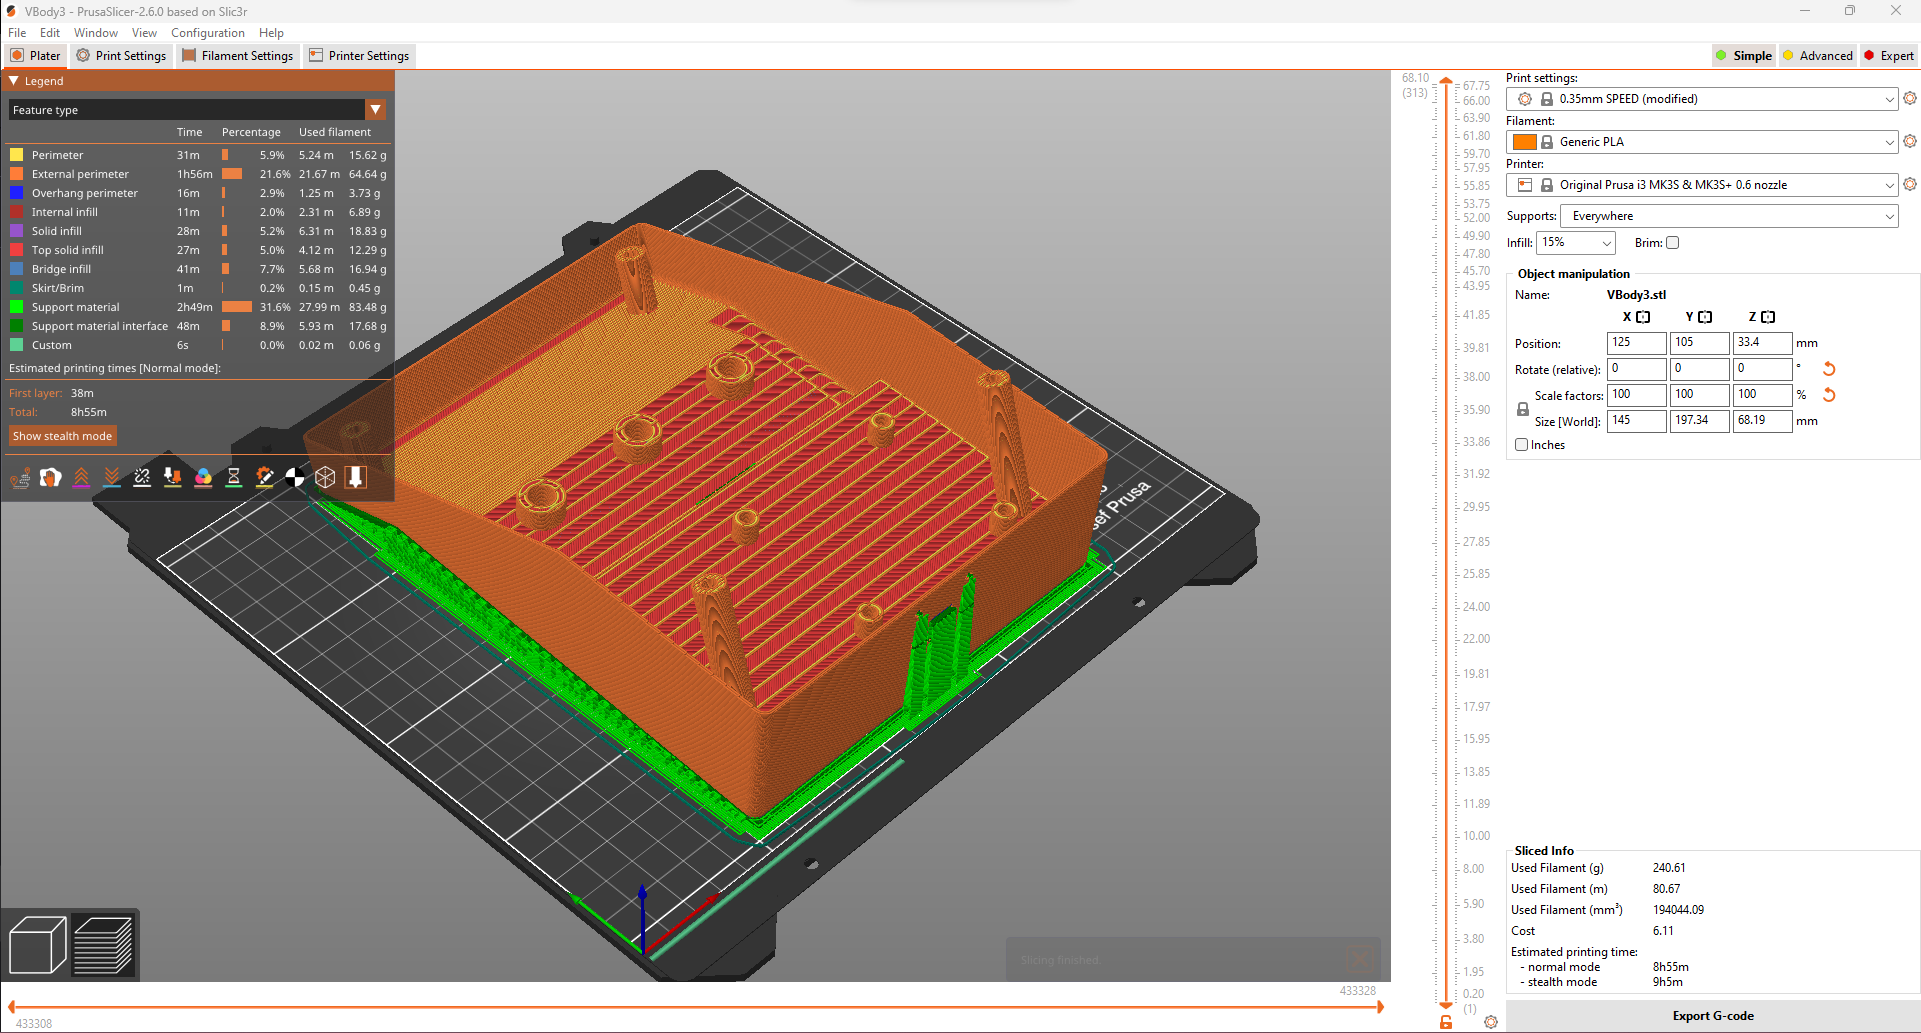
\includegraphics[width=0.8\linewidth]{texs/Part1/chapter1/image/prusaslicer.png}
    \caption{Example View of PrusaSlicer}
    \label{fig:prusa_slicer}
\end{figure}


\subsection{Printing Cost}
\label{subsec:printing_cost}

To perform a cost analysis of the 3D printing process, we will consider the following parameters:

\begin{itemize}
    \item Material Cost
    \item Energy Cost
\end{itemize}

Material cost refers to the cost of the filament used in the printing process. The filament is the material that is deposited layer by layer to create the final product. The cost of the filament is dependent on the type of material used. For this project, we will be using PLA, which costs 29.99 € per kilogram \cite{PrusaCost}.

The amount of filament used in the printing process is dependent on the size of the object being printed. The PrusaSlicer software provides an estimate of the amount of filament required for a given object.

Energy cost refers to the cost of electricity used in the printing process. The amount of electricity used is dependent on the duration of the printing process. The PrusaSlicer software provides an estimate of the duration of the printing process.

Equation \ref{eq:printing_cost} shows the formula for calculating the cost of 3D printing.

\begin{equation}
    \label{eq:printing_cost}
    C_{print} = m_{f}\cdot C_{f}+t_{p}\cdot C_{e}
\end{equation}

where $C_{print}$ is the printing cost, $m_{f}$ is the mass of filament used, $C_{f}$ is the cost of filament, $t_{p}$ is the duration of printing process, and $C_{e}$ is the cost of electricity.


